% Gemini theme
% https://github.com/anishathalye/gemini
% We try to keep this Overleaf template in sync with the canonical source on
% GitHub, but it's recommended that you obtain the template directly from
% GitHub to ensure that you are using the latest version.

% Brown University color schemes for Gemini theme
% https://github.com/vskbellala/gemini-brown

\documentclass[final]{beamer}

% ====================
% Packages
% ====================

\usepackage[T1]{fontenc}
\usepackage{lmodern}
\usepackage[size=custom,width=96,height=72,scale=1.0]{beamerposter}
\usetheme{gemini}
\usecolortheme{brown}
% \usecolortheme{brownminimal}
\usepackage{graphicx}
\usepackage{booktabs}
\usepackage{tikz}
\usepackage{pgfplots}
\pgfplotsset{compat=1.14}

% ====================
% Lengths
% ====================

% If you have N columns, choose \sepwidth and \colwidth such that
% (N+1)*\sepwidth + N*\colwidth = \paperwidth
\newlength{\sepwidth}
\newlength{\colwidth}
\setlength{\sepwidth}{0.025\paperwidth}
\setlength{\colwidth}{0.3\paperwidth}

\newlength{\rightwide}
\setlength{\rightwide}{\dimexpr 2\colwidth+\sepwidth\relax}


\newcommand{\separatorcolumn}{\begin{column}{\sepwidth}\end{column}}

% ====================
% Title
% ====================

\title{Learning Minimal-Fuel Corrections for the Figure-8 Orbit}

\author{Ignacio Blancas Rodriguez \inst{1} \and Ryan L Yang \inst{1} \and Patrick Verma \inst{1}}

\institute[shortinst]{\inst{1} Brown University}

% ====================
% Footer (optional)
% ====================

% \footercontent{
%   \href{https://www.example.com}{https://www.example.com} \hfill
%   ABC Conference 2025, New York --- XYZ-1234 \hfill
%   \href{mailto:alyssa.p.hacker@example.com}{alyssa.p.hacker@example.com}}
% (can be left out to remove footer)

% ====================
% Logo (optional)
% ====================

% use this to include logos on the left and/or right side of the header:
% \logoright{\includegraphics[height=7cm]{logo1.pdf}}
\logoleft{\includegraphics[height=7cm]{images/Brown_white.png}}
% \logoleft{\includegraphics[height=7cm]{images/Brown_full.png}}


% ====================
% Body
% ====================

\begin{document}

\begin{frame}[t]
\begin{columns}[t]
\separatorcolumn

\begin{column}{\colwidth}

  \begin{block}{Problem statement}

    The $N$-body problem considers three planetary bodies and the evolution of their positions and velocities over time under their gravitational interactions. For $N \geq 3$ there is no closed form solution and the solutions may become chaotic. We consider a 3-agent RL setup, where each agent is able to apply an $a_i$ acceleration to the $i$-th body every $\Delta T$ time-step. The goal is for the agents to learn minimal $a_i$ pushes to get the three bodies in some target stable orbit, for example, the Figure-8 orbit.

  \end{block}

  \begin{block}{Architecture Description}

    In order for the independent actors to learn coordinated actions we train the independent agents via a centralized critic and reward function. We break our system down into the following layers,

    \begin{itemize}
      \item \textbf{Physics environment:} a numerical 3-body simulator updates
      positions and velocities using the agents' thrust actions and gravitational
      interactions.

      \item \textbf{Graph encoder:} A GNN, where each body corresponds to a node and edges encode their gravitational interactions, produces three embedding vectors $h_i$ one for each body.

      \item \textbf{Decentralized actors:} Each actor is given an embedding $h_i$ and produces an acceleration vector $a_i$ that will be applied to the $i$-th body for $\Delta T$ time.

      \item \textbf{Centralized critic and reward:} During training, a global
      critic observes the full system state and joint action. The reward combines
      orbit-position error, velocity error, fuel penalty, survival rewards, phase synchronization, and stable permutation of the bodies.
    \end{itemize}

  \end{block}

  \begin{alertblock}{The reward function}

    Our simulation implements the following reward function,
    $$
    R = \omega_{o} R_{o}  + \omega_{f} R_f + \omega_{s} R_s + \omega_p R_p + \omega_\text{perm} R_\text{perm}
    $$
    where each $\omega$ represents the weight 

  \end{alertblock}

  \begin{figure}
  \centering
  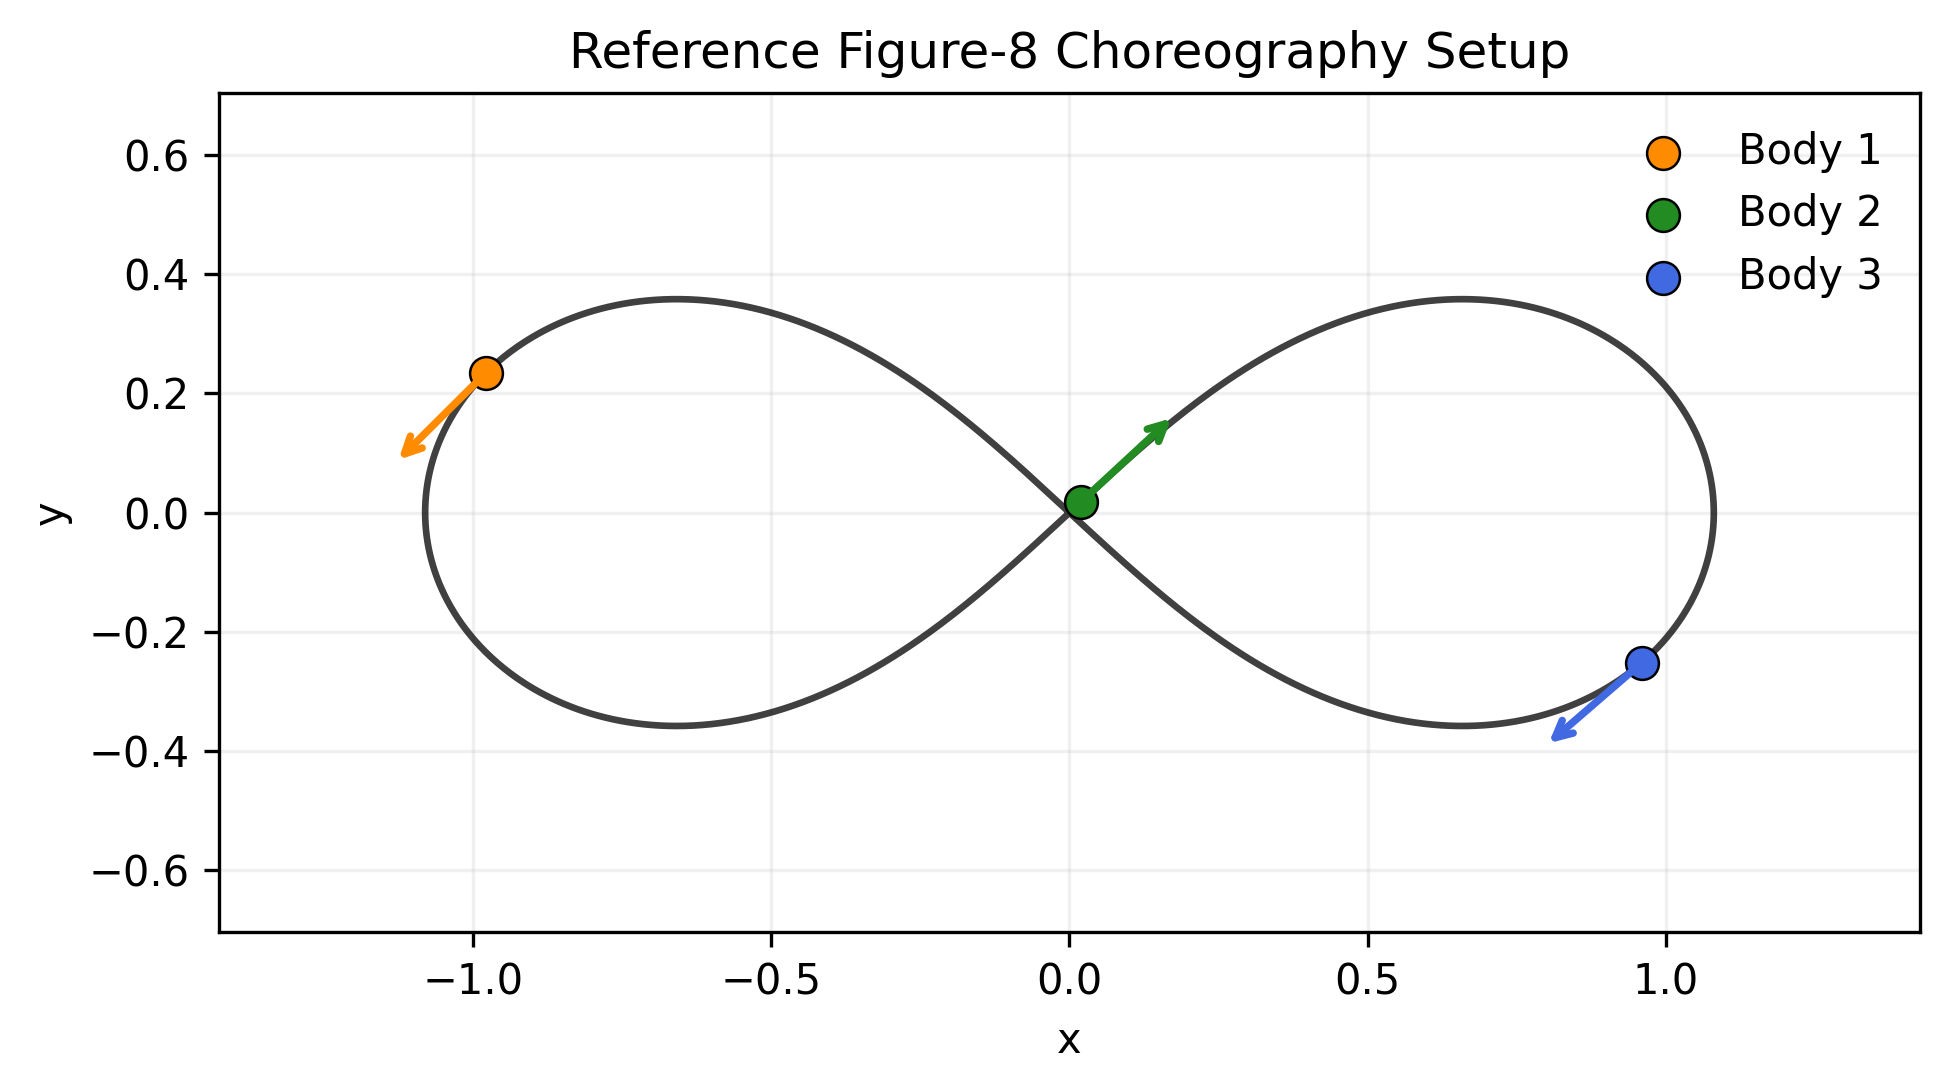
\includegraphics[width=0.88\linewidth]{figures/reference_figure8_paper.png}
  \caption{Reference Figure-8 choreography. The stored target orbit provides
  position and velocity targets for matching the simulated state at each step.}
\end{figure}


\end{column}

\separatorcolumn

\begin{column}{\rightwide}

  \begin{columns}[t,totalwidth=\rightwide]

    \begin{column}{\colwidth}

      \begin{block}{Matching the state to the target orbit}

        We store the Figure-8 as reference snapshots: where each body should be
        and which direction it should move at each point in the choreography.
        Because the bodies have equal mass, their labels are interchangeable.
        At each step, the environment tries every assignment between simulated
        bodies and reference bodies, then chooses the best match.

        The match uses four criteria:

        \begin{itemize}
          \item \textbf{Position:} bodies should be close to the reference locations.

          \item \textbf{Velocity direction:} bodies should move in the same direction
          as the reference choreography.

          \item \textbf{Phase continuity:} the matched point on the Figure-8 should
          move smoothly forward over time.

          \item \textbf{Assignment continuity:} the same simulated body should keep
          matching the same reference track unless switching gives a much better fit.
        \end{itemize}

        The assignment-continuity penalty prevents the matcher from rapidly
        swapping body identities between frames. This makes the reward reflect a
        cleaner physical choreography, where each body settles into a consistent
        role in the Figure-8 motion.

      \end{block}

      \begin{block}{Initial Positions}

        Fully random starts made the task too difficult: most episodes quickly
        produced collisions, escapes, or states far from the Figure-8. We
        therefore use \textbf{directed initialization}: start from one fixed
        configuration near the target choreography, then add small random
        perturbations to positions and velocities.

        This keeps training near the orbit we care about while still preventing
        the policy from memorizing one exact trajectory. The agents learn local
        corrective pushes that stabilize the Figure-8 while keeping fuel usage
        small.

      \end{block}

    \end{column}

    \separatorcolumn

    \begin{column}{\colwidth}

  % \begin{exampleblock}{A highlighted block containing some math}

  %   A different kind of highlighted block.

  %   $$
  %   \int_{-\infty}^{\infty} e^{-x^2}\,dx = \sqrt{\pi}
  %   $$

  %   Interdum et malesuada fames $\{1, 4, 9, \ldots\}$ ac ante ipsum primis in
  %   faucibus. Cras eleifend dolor eu nulla suscipit suscipit. Sed lobortis non
  %   felis id vulputate.

  %   \heading{A heading inside a block}

  %   Praesent consectetur mi $x^2 + y^2$ metus, nec vestibulum justo viverra
  %   nec. Proin eget nulla pretium, egestas magna aliquam, mollis neque. Vivamus
  %   dictum $\mathbf{u}^\intercal\mathbf{v}$ sagittis odio, vel porta erat
  %   congue sed. Maecenas ut dolor quis arcu auctor porttitor.

  %   \heading{Another heading inside a block}

  %   Sed augue erat, scelerisque a purus ultricies, placerat porttitor neque.
  %   Donec $P(y \mid x)$ fermentum consectetur $\nabla_x P(y \mid x)$ sapien
  %   sagittis egestas. Duis eget leo euismod nunc viverra imperdiet nec id
  %   justo.

  % \end{exampleblock}

  \begin{block}{Training and Challenges}

    Class aptent taciti sociosqu ad litora torquent per conubia nostra, per
    inceptos himenaeos. Phasellus libero enim, gravida sed erat sit amet,
    scelerisque congue diam. Fusce dapibus dui ut augue pulvinar iaculis.

    \begin{table}
      \centering
      \begin{tabular}{l r r c}
        \toprule
        \textbf{First column} & \textbf{Second column} & \textbf{Third column} & \textbf{Fourth} \\
        \midrule
        Foo & 13.37 & 384,394 & $\alpha$ \\
        Bar & 2.17 & 1,392 & $\beta$ \\
        Baz & 3.14 & 83,742 & $\delta$ \\
        Qux & 7.59 & 974 & $\gamma$ \\
        \bottomrule
      \end{tabular}
      \caption{A table caption.}
    \end{table}

    Donec quis posuere ligula. Nunc feugiat elit a mi malesuada consequat. Sed
    imperdiet augue ac nibh aliquet tristique. Aenean eu tortor vulputate,
    eleifend lorem in, dictum urna. Proin auctor ante in augue tincidunt
    tempor. Proin pellentesque vulputate odio, ac gravida nulla posuere
    efficitur. Aenean at velit vel dolor blandit molestie. Mauris laoreet
    commodo quam, non luctus nibh ullamcorper in. Class aptent taciti sociosqu
    ad litora torquent per conubia nostra, per inceptos himenaeos.

    Nulla varius finibus volutpat. Mauris molestie lorem tincidunt, iaculis
    libero at, gravida ante. Phasellus at felis eu neque suscipit suscipit.
    Integer ullamcorper, dui nec pretium ornare, urna dolor consequat libero,
    in feugiat elit lorem euismod lacus. Pellentesque sit amet dolor mollis,
    auctor urna non, tempus sem.

  \end{block}




  \begin{block}{References}

    \nocite{*}
    \footnotesize{\bibliographystyle{abbrv}\bibliography{poster}}

  \end{block}

    \end{column}

  \end{columns}

  \vspace{1cm}

  \begin{figure}
    \centering
    
\includegraphics[width=0.96\linewidth]{figures/policy_push_correction.png}
    \caption{Directed initialization and policy correction. The policy learns
    small thrusts that move perturbed states toward the Figure-8 while penalizing
    larger fuel usage.}
  \end{figure}

\end{column}


\separatorcolumn
\end{columns}





\end{frame}

\end{document}
